% LaTex Template

\documentclass[12pt]{article}
%\usepackage{natbib}
\usepackage[letterpaper, margin=1.1in]{geometry}
\usepackage{graphicx}
\usepackage{wrapfig}
\usepackage{enumitem}
\setlist[enumerate]{itemsep=0mm}
\usepackage{multirow}
\usepackage[table,xcdraw]{xcolor}
\usepackage{lscape}
\usepackage{caption}
\usepackage{subcaption}
\usepackage{hyperref}

\newcommand{\transectAbb}{Data for each glacier are divided into lower hourglass (LH), lower circle (LC), lower midline (LM), upper hourglass (UH), upper circle (UC), upper midline (UM), and upper transect (UT).}

\begin{document}
\noindent{Alexandra Pulwicki \\ \today}

\begin{center}
\Large \textbf{Results\\ Point Scale}
\end{center}


\tableofcontents
\pagebreak



\begin{wraptable}[29]{R}{8cm}
\centering
\caption{Normality of data with various subgroups. $\chi^2$ values are shown and normally distributed data is bold ($p<0.05$). \transectAbb}
\label{tab:normality}
\begin{tabular}{cccc}
\textbf{Glacier} & \textbf{Transect} & \multicolumn{2}{c}{\textbf{$\chi^2$}} \\ 
\hline
\hline 
& LH & 14.9 &   \\
  & LC & 17.3 &   \\
  & LM & 6.6 &   \\
  & UH & 52.1 &   \\
  & UC & \textbf{5.9} &   \\
& UM & \textbf{1.4} &   \\
\multirow{-7}{*}{Glacier 4} & UT & 15.7 & \multirow{-7}{*}{ 115.4} \\ \hline
 & LH & 27.8 &  \\
 & LC & \textbf{5.0} &  \\
 & LM & \textbf{6.2} &  \\
 & UH & 43.8 &  \\
 & UC & 13.1 &  \\
 & UM & 31.3 &  \\
 & UT & \textbf{0.1} &  \\
\multirow{-8}{*}{Glacier 2} & BT & 13.1 & \multirow{-8}{*}{127.1} \\ \hline
  
  & LH & 32.1 &   \\ 
  
  & LC & 11.4 &   \\
  
  & LM & 18.1 &   \\
  
  & UH & 12.8 &   \\
  
  & UC & 17.6 &   \\
  
  & UM & 9.7 &   \\
  
\multirow{-7}{*}{ Glacier 13} & UT & 8.6 & \multirow{-7}{*}{ 39.4}
\end{tabular}
\end{wraptable}

\section{Point Scale}

This section details basic statistical results of the snow depth data at the point scale. The goal of these analyses is to examine variability of single measurements and to determine whether any correction need to be made to the collected data for future analysis. First, the normality of snow depth measurements is examined. Then, the effect of different observers on snow depth measurement is examined. In Section 3, the mean and overall standard deviations are compared. The final section examines the variability as a function of elevation on the three study glaciers. 

\subsection{Data normality}

A $\chi^2$ test is done to test whether the collected snow depth data are normally distributed. Generally, the transect snow depth data are not normally distributed and are even further from normality (larger $\chi^2$ values) for data grouped by glacier (Table \ref{tab:normality}). However, we chose to not transform the data in order to maintain its original context and because transformation of snow depth data is not typically done.  

\subsection{Observer differences}

An ANOVA for each transect of snow depth measurements taken by different observers shows that there are no differences between observers (p $>$ 0.05) (data not shown). The only exception is the Lower Hourglass on Glacier 4, where snow depth values collected by one observer were, on average, greater than the snow depth measurements taken by the other two observers ( AC$>$AP=CA with p $<$ 0.01). Since this was the first transect completed and the only one to show differences by observer, this difference can be considered an anomaly. This result shows that observer bias is likely to not affect the results of this study and no corrections to the data based on observer were applied.

\subsection{Standard deviation of snow depth along linear and curvilinear transects}

\begin{wrapfigure}[26]{l}{0.7\textwidth} 
\centering
	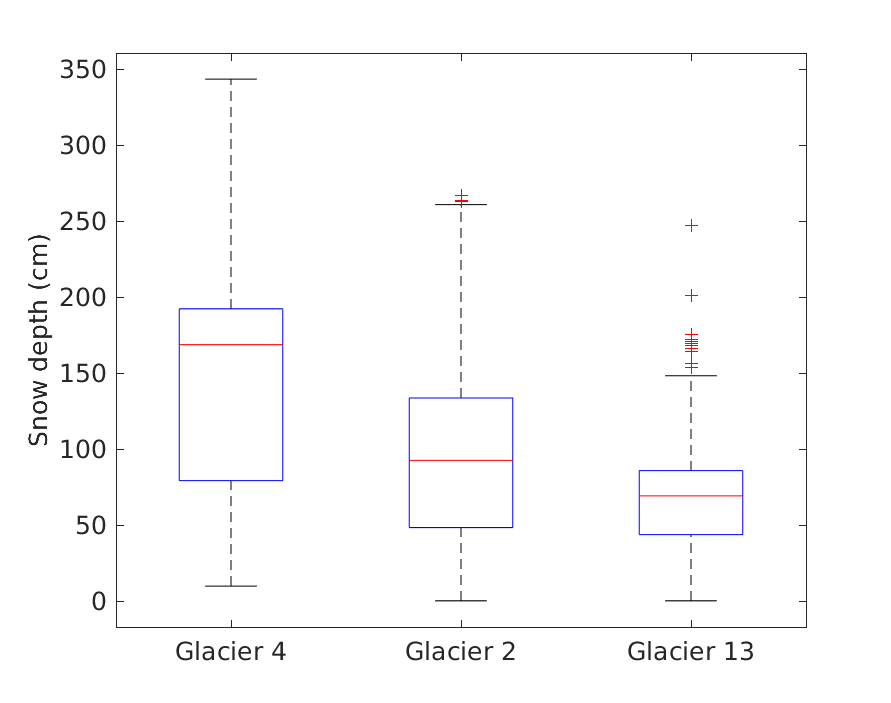
\includegraphics[width = 0.7\textwidth]{box_depth.png}\\
	\caption{Variability in all snow depth measurements taken at each glacier. Red line indicates median, blue box shows first quantiles, bars indicate minimum and maximum values (excluding outliers), and red crosses show outliers, which are defined as being outside of the range of 1.5 times the quartiles (approximately $\pm2.7\sigma$).}
	\label{fig:box_depth}
\end{wrapfigure}

The mean standard deviation of snow depth measurements collected at each location within various transects was found by calculating the standard deviation of the three to four measurements made by each observer at each measurement location (Table \ref{tab:std_reproduce}. The mean of these standard deviations for each grouping (Table \ref{tab:std_reproduce}) represents the variability in snow depth for the sampling locations. It can be used to evaluate the representativeness of the mean snow depth values that were used in the analysis at larger scales.

The overall standard deviation of all measurements was calculated by taking all the depth measurements within a subset of the data and then calculating the standard deviation (Table \ref{tab:std_measure}). The overall standard deviation represents the variability in the depth field. 

The mean standard deviation varies between glaciers, transects, and observers but  generally, the reproducibility of depth measurement is on the order of centimetres (10$^0$). The overall standard deviation of measurements over the study area is on the order of 10$^1$. Therefore, the standard deviation of a snow depth measurement is small compared to the standard deviation of all snow depth measurements. When expressed as a percentage of the mean, the overall standard deviation (Table \ref{tab:std_measure}) is also larger than that of the mean standard deviation (Table \ref{tab:std_reproduce}). This shows that variability at the point scale (a single measurement location) is an order of magnitude smaller than the variability of the depth field for the length of a transect, so the use of the mean snow depth at each measurement location is a valid value to carry forward in the analysis. 

Variability in snow depth differs considerably between glaciers (Figure \ref{fig:box_depth}). Both the range and mean depth are largest for Glacier 4 and smallest for Glacier 13. Glacier 13 has the most outliers (\textgreater 1.5 $\times$ inner quartile range). The standard deviation of all measurement taken on a glacier (Table \ref{tab:std_measure}) is lowest for Glacier 13 and highest for Glacier 2, with the standard deviation of Glacier 4 being close to that of Glacier 2. 

The standard deviation as a function of binned elevation show that the standard deviation decreases with elevation on both Glacier 2 and 13 but it increases with elevation on Glacier 4 (Figure \ref{fig:std_snowdepth_binned}). The regression of elevation and standard deviation as percent of the mean is strong for Glacier 2 (R$^2$ = 0.79) and weak for Glacier 13 (R$^2$ = 0.38) and Glacier 4 (R$^2$ = 0.12). Therefore, the variability is higher closer to the terminus of the Glacier 2 and there is no significant trend on Glacier 4 and 13. However, there are comparatively fewer depth measurements taken at higher elevations, which may skew the trend of higher variability close to the terminus. 


%% Std of reproducibility
\begin{table}[h]
\footnotesize
\centering
\caption{Mean standard deviation (cm) of snow depth measurements for the entire glacier (Overall Glacier), different transects (Overall Transect), and each observer. Standard deviation as a percent of the mean snow depth is shown in brackets. \transectAbb}
\label{tab:std_reproduce}
\begin{tabular}{cccccccc}
 &  &  &  & \multicolumn{4}{c}{\textbf{Observer}} \\
\multirow{-2}{*}{} & \multirow{-2}{*}{\textbf{Transect}} & \multirow{-2}{*}{\textbf{\begin{tabular}[c]{@{}c@{}}Overall \\ Glacier\end{tabular}}} & \multirow{-2}{*}{\textbf{\begin{tabular}[c]{@{}c@{}}Overall \\ Transect\end{tabular}}} & AP & GF & CA & AC \\ \hline \hline
  
  & LH &   & 5.1 (3\%)& 4.8  (3\%)& --- & 8.5 (5\%) & 2.0 (1\%) \\
  
  & LC &   & 4.7  (3\%)& 4.3  (3\%)& --- & 8.2  (5\%)& 1.7  (1\%)\\
  
  & LM &   & 3.7  (2\%)& --- & 4.7  (3\%)& 4.6  (2\%)& 1.9  (1\%)\\
  
  & UH &   & 2.6   (1\%)& 3.4   (1\%)& 2.2   (1\%)& --- & 2.3   (1\%)\\
  
  & UC &   & 1.9   (1\%)& 1.9   (2\%)& 2.3   (1\%)& --- & 1.5  (1\%) \\
  
  & UM &   & 1.9   (1\%)& --- & 1.7   (1\%)& 2.0 (1\%) & 2.0 (1\%)\\
  
\multirow{-7}{*}{ Glacier 4} & UT & \multirow{-7}{*}{ 3.5 (2\%)} & 3.9 (2\%)& 3.7 (2\%) & --- & 2.4 (1\%)& 5.6 (3\%)\\ \hline
 & LH &  & 5.4 (11\%)& 4.8 (9\%)& --- & 6.1 (13\%)& --- \\ 
 & LC &  & 5.0 (12\%)& 3.9 (11\%)& --- & 6.2 (15\%)& --- \\
 & LM &  & 6.5 (17\%)& --- & 6.8 (16\%)& 6.5 (18\%)& 6.0 (16\%)\\
 & UH &  & 4.1 (7\%)& 3.5 (5\%)& 4.4 (7\%)& 4.5 (9\%)& --- \\
 & UC &  & 7.0 (4\%)& 5.5 (3\%)& 7.0 (4\%)& 8.7 (4\%)& --- \\
 & UM &  & 4.2 (4\%)& 3.2 (3\%)& 5.2 (4\%)& 4.1 (4\%)& --- \\
 & UT &  & 5.6 (10\%)& 3.2 (6\%)& --- & 8.2 (13\%)& --- \\
\multirow{-8}{*}{Glacier 2} & BT & \multirow{-8}{*}{5.1 (7\%)} & 2.2 (2\%)& 2.2 (2\%)& --- & 3.0 (2\%)& 1.5 (1\%) \\ \hline
  
  & LH &   & 3.8 (10\%)& 3.1 (6\%)& 4.1 (12\%) & 4.0 (13\%)& --- \\ 
  
  & LC &   & 4.5 (8\%)& 2.9 (6\%)& 4.8 (9\%)& 5.8 (8\%)& --- \\
  
  & LM &   & 6.6 (13\%)& 4.6 (10\%)& 7.7 (16\%)& 7.6 (14\%)& --- \\
  
  & UH &   & 3.5 (4\%)& 3.4 (4\%)& 3.6 (5\%)& 3.4 (5\%)& --- \\
  
  & UC &   & 3.8 (4\%)& 3.4 (4\%)& 4.0 (4\%)& 4.0 (4\%)& --- \\
  
  & UM &   & 4.8 (6\%)& 4.4 (5\%)& 5.8 (7\%) & 4.4 (5\%) & --- \\
  
\multirow{-7}{*}{ Glacier 13} & UT & \multirow{-7}{*}{ 4.2 (6\%)} & 4.1 (6\%)& 2.7 (4\%)& 4.8 (6\%)& 4.6 (7\%)& ---
\end{tabular}
\end{table}


%% Std of measurement
\begin{table}[]
\footnotesize
\centering
\caption{Overall standard deviation (cm) of snow depth measurements for the entire glacier (Overall Glacier), different transects (Overall Transect), and each observer. Standard deviation as a percent of the mean snow depth is shown in brackets. \transectAbb The standard deviation of all transect data was 64.6 cm.}
\label{tab:std_measure}
\begin{tabular}{cccccccc}
 &  &  &  & \multicolumn{4}{l}{\textbf{Person}} \\
\multirow{-2}{*}{\textbf{Glacier}} & \multirow{-2}{*}{\textbf{Pattern}} & \multirow{-2}{*}{\textbf{\begin{tabular}[c]{@{}l@{}}Overall \\ Glacier\end{tabular}}} & \multirow{-2}{*}{\textbf{\begin{tabular}[c]{@{}l@{}}Overall \\ Pattern\end{tabular}}} & AP & GF & CA & AC \\ \hline \hline
  
  & LH &   & 51.3  (28\%)& 51.4  (29\%) & --- & 54.8  (32\%) & 45.7  (24\%) \\
  
  & LC &   & 45.2  (26\%) & 50.5  (30\%) & --- & 44.1  (25\%) & 39.8  (23\%) \\
  
  & LM &   & 27.2  (15\%) & --- & 21.6   (11\%)& 36.3  (19\%) & 22.5  (12\%) \\
  
  & UH &   & 48.5  (28\%) & 48.6  (28\%) & 51.2   (29\%)& --- & 45.8  (27\%) \\
  
  & UC &   & 44.2  (23\%) & 44.8  (23\%) & 38.2   (21\%)& --- & 48.2   (26\%)\\
  
  & UM &   & 22.5  (13\%) & --- & 24.1  (14\%) & 20.7  (12\%) & 22.7  (13\%) \\
  
\multirow{-7}{*}{ Glacier 4} & UT & \multirow{-7}{*}{ 44.7  (25\%)} & 26.0   (13\%)& 25.1  (13\%) & --- & 25.1  (13\%) & 27.7  (14\%) \\ \hline
 & LH &  & 29.9  (67\%) & 29.2  (63\%) & --- & 30.6  (71\%) & --- \\
 & LC &  & 29.3  (61\%) & 28.6  (63\%) & --- & 30.1  (59\%) & --- \\
 & LM &  & 18.4  (43\%) & --- & 20.8   (45\%)& 15.5  (39\%) & 18.1  (43\%) \\
 & UH &  & 42.0  (39\%) & 39.1  (37\%) & 41.6  (38\%) & 45.6  (42\%) & --- \\
 & UC &  & 55.0   (52\%)& 55.3  (53\%) & 55.2  (52\%) & 56.1  (52\%) & --- \\
 & UM &  & 35.1  (29\%) & 38.4  (33\%) & 34.5  (29\%) & 31.8  (27\%) & --- \\
 & UT &  & 36.4  (61\%) & 27.3 (51\%) & --- & 43.9  (70\%) & --- \\
\multirow{-8}{*}{Glacier 2} & BT & \multirow{-8}{*}{49.3 (62\%)} & 20.8 (14\%)& 13.8 (10\%)& --- & 13.7 (9\%) & 30.4 (22\%) \\ \hline
  
  & LH &   & 27.4  (56\%) & 25.7 (53\%) & 27.5 (58\%) & 28.9 (57\%) & --- \\
  
  & LC &   & 27.1  (59\%) & 25.8 (57\%) & 21.4 (52\%) & 32.6 (68\%) & --- \\
  
  & LM &   & 24.9  (52\%) & 22.8 (60\%) & 27.5 (56\%) & 23.6 (42\%) & --- \\
  
  & UH &   & 21.0  (25\%) & 21.1 (25\%) & 21.4 (25\%) & 20.4 (24\%) & --- \\
  
  & UC &   & 16.3  (18\%) & 17.6 (21\%) & 14.5 (16\%) & 16.6 (18\%) & --- \\
  
  & UM &   & 29.4  34(\%) & 26.6 (32\%) & 33.4 (39\%) & 28.0 (33\%) & --- \\
  
\multirow{-7}{*}{ Glacier 13} & UT & \multirow{-7}{*}{ 30.5 (46\%)} & 32.7 (50\%) & 21.5 (31\%) & 44.4 (63\%) & 26.4 (42\%) & ---
\end{tabular}
\end{table}


\begin{figure}
    \centering
    \begin{subfigure}[b]{0.8\textwidth}
        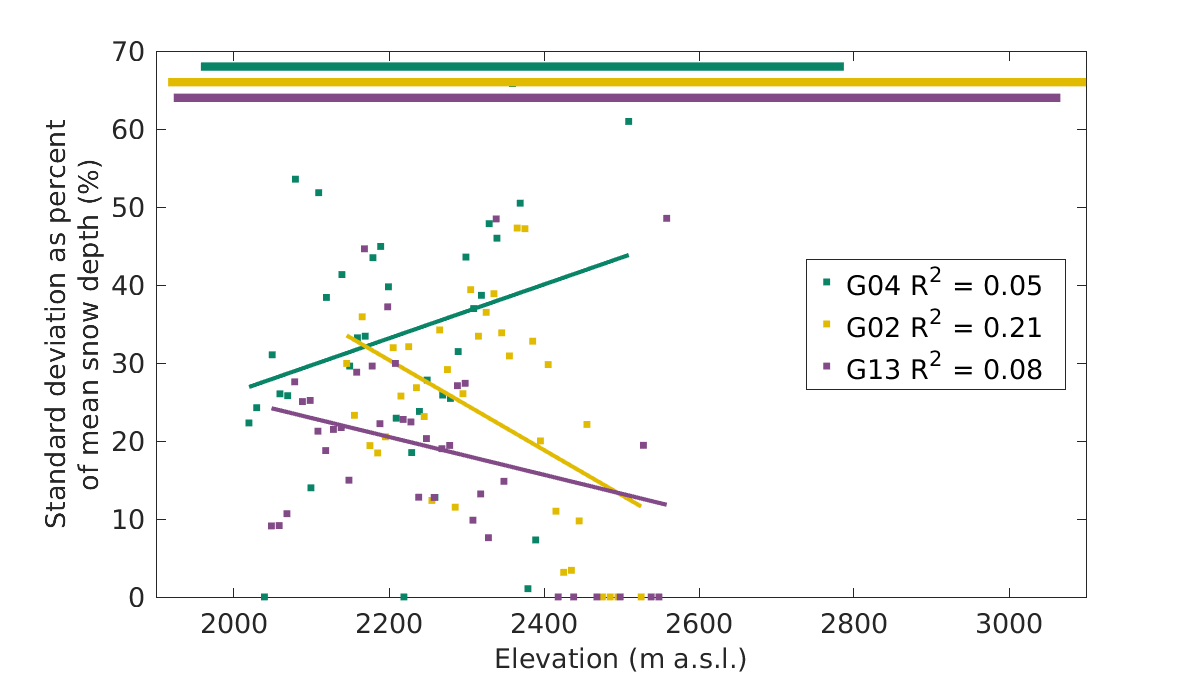
\includegraphics[width=\textwidth]{binned_std.png}
        \caption{}
    \end{subfigure}
    
    \begin{subfigure}[b]{0.8\textwidth}
        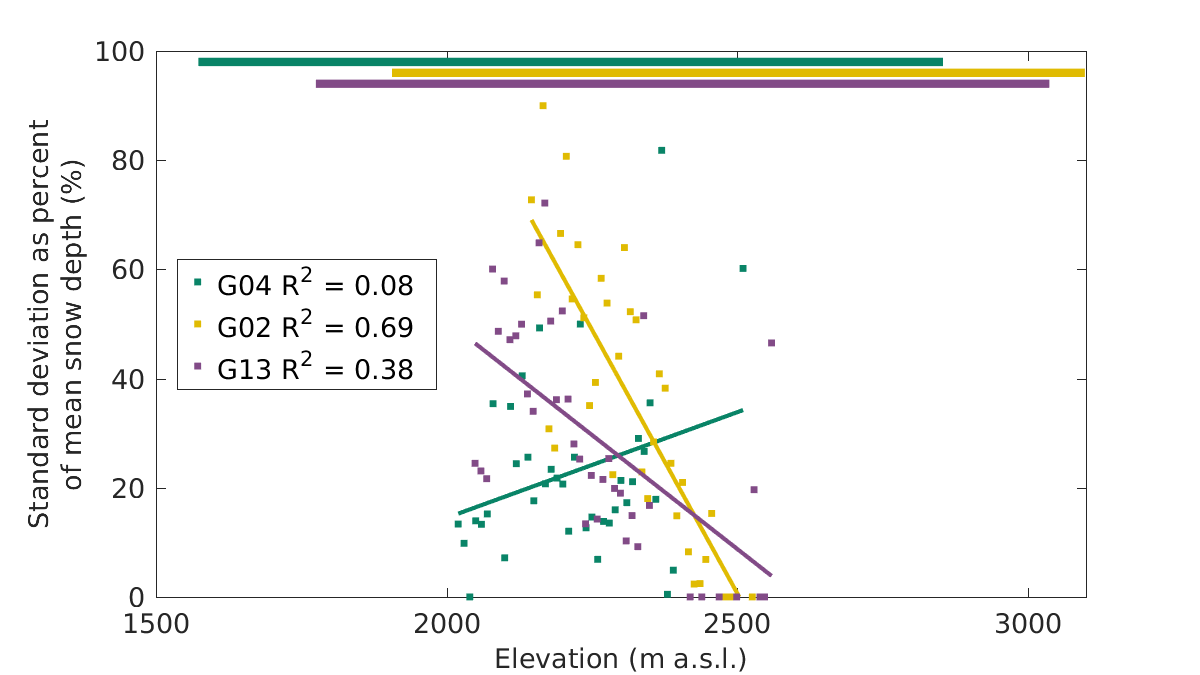
\includegraphics[width=\textwidth]{binned_std_percent.png}
        \caption{}
    \end{subfigure}

    \caption{Standard deviation (a) and standard deviation as percent of mean (b) of all snow depth measurements binned in elevation bands of 10 m. Bars at the top of the figure indicate the elevation ranges of the three study glaciers. The regression of elevation and standard deviation of snow depth is shown as a coloured line within the data.}
    \label{fig:std_snowdepth_binned}
\end{figure}











\end{document}
